\chapter{Исследовательская часть}

В данном разделе будут приведены примеры работы программы, и будет проведен сравнительный анализ реализованных алгоритмов умножения матриц по затраченному процессорному времени.

\section{Технические характеристики}

Тестирование проводилось на устройстве со следующими техническими характеристиками:

\begin{itemize}
	\item операционная система: Ubuntu 20.04.1 Linux x86\_64 \cite{linux};
	\item память : 8 GiB;
	\item процессор: AMD® Ryzen™ 3 3200u @ 2.6 GHz \cite{amd}.
\end{itemize}

Тестирование проводилось на ноутбуке, включенном в сеть электропитания. Во время тестирования ноутбук был нагружен только встроенными приложениями окружения, а также непосредственно системой тестирования.

\clearpage

\section{Демонстрация работы программы}

На рисунке \ref{img:example} приведен пример работы программы.

\begin{figure}[H]
	\begin{center}
		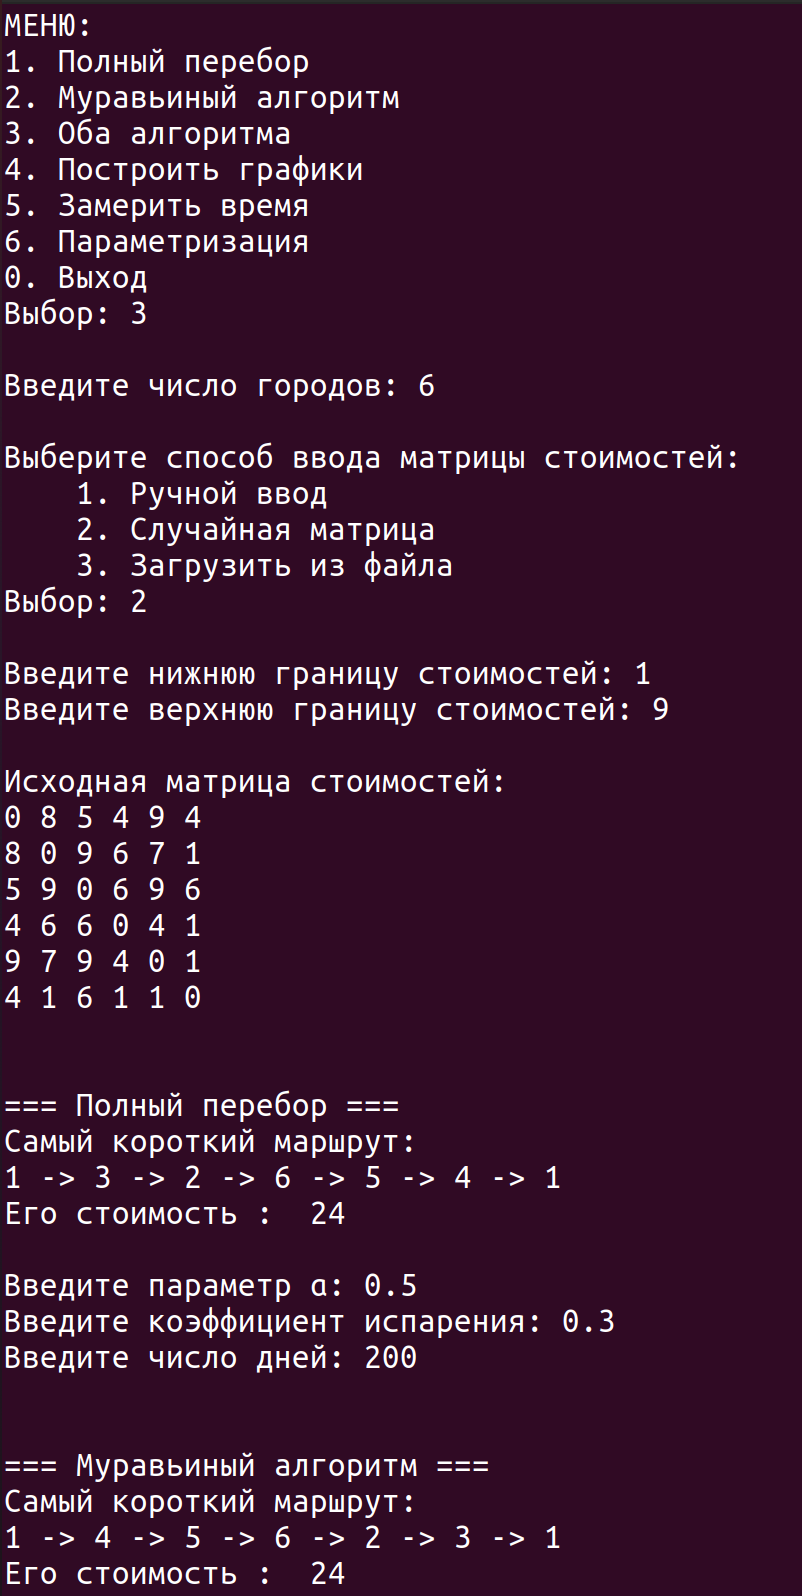
\includegraphics[scale=0.3]{img/example.png}
	\end{center}
	\captionsetup{justification=centering}
	\caption{Пример работы программы}
	\label{img:example}
\end{figure}

\section{Время выполнения алгоритмов}

Функция process\_time из библиотеки time ЯП Python возвращает  процессорное время в секундах - значение типа float.

Для замера времени необходимо получить значение времени до начала выполнения алгоритма, затем после её окончания. Чтобы получить результат, необходимо вычесть из второго значения первое.

Замеры проводились для матриц стоимостей, заполненных случайным образом, размером от 2 до 10. Результаты измерения времени приведены в таблице \ref{tbl:time} (в с), а их графическое представление - на рисунке \ref{img:time}.

\begin{center}
\captionsetup{justification=raggedright,singlelinecheck=off}
\begin{longtable}[c]{|p{4cm}|p{4cm}|p{4cm}|}
\caption{Результаты замеров времени\label{tbl:time}}\\ \hline
   Число городов & Полный перебор & Муравьиный алгоритм \\ \hline
   2 &   0.000327 &   0.010621 \\ \hline
   3 &   0.000039 &   0.015454 \\ \hline
   4 &   0.000121 &   0.031155 \\ \hline
   5 &   0.000706 &   0.049366 \\ \hline
   6 &   0.003409 &   0.078147 \\ \hline
   7 &   0.024055 &   0.106820 \\ \hline
   8 &   0.223502 &   0.149278 \\ \hline
   9 &   2.248946 &   0.227690 \\ \hline
  10 &  22.530937 &   0.299644 \\ \hline
\end{longtable}
\end{center}

\begin{figure}[H]
	\begin{center}
		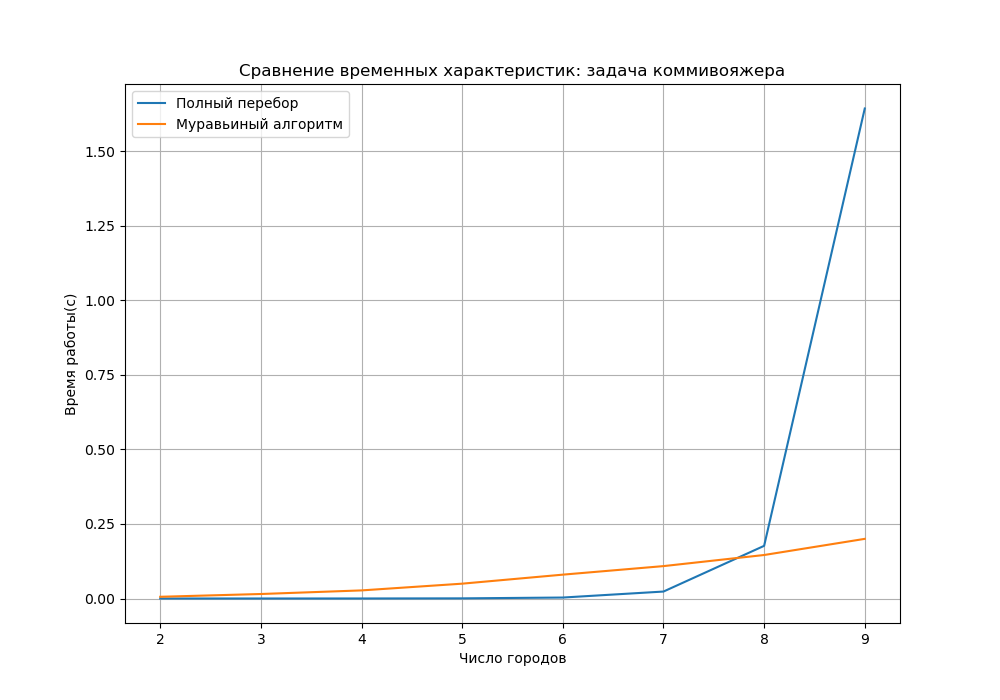
\includegraphics[scale=0.5]{img/time.png}
	\end{center}
	\captionsetup{justification=centering}
	\caption{Сравнение по времени алгоритмов задачи коммивояжера}
	\label{img:time}
\end{figure}

\section{Параметризация}

Целью проведения параметризации является определение таких комбинаций параметров, при которых муравьиный алгоритм даёт наилучшие результаты.

В результате автоматической параметризации будет получена таблицы со следующими столбцами:
\begin{itemize}
	\item коэффициент видимости $\alpha$ - изменяющийся параметр;
	\item коэффициент испарения феромона $\rho$ - изменяющийся параметр;
	\item число дней $days$ - изменяющийся параметр;
	\item эталонный результат $ideal$;
	\item разность полученного при данных параметрах значения и эталонного $mistake$.
\end{itemize}

\subsection{Класс данных 1}

Класс данных 1 представляет собой матрицу стоимостей в диапозоне от 1 до 5 для 8 городов:

\begin{equation}
    \label{eq:kd1}
	K_{1} = \begin{pmatrix}
		0 & 4 & 3 & 2 & 4 & 5 & 5 & 3 \\
		4 & 0 & 4 & 5 & 5 & 1 & 4 & 5 \\
		3 & 4 & 0 & 5 & 4 & 1 & 2 & 1 \\
		2 & 5 & 5 & 0 & 1 & 3 & 1 & 5 \\
		4 & 5 & 4 & 1 & 0 & 2 & 5 & 4 \\
		5 & 1 & 1 & 3 & 2 & 0 & 4 & 5 \\
		5 & 4 & 2 & 1 & 5 & 4 & 0 & 2 \\
		3 & 5 & 1 & 5 & 4 & 5 & 2 & 0 \\
	\end{pmatrix}
\end{equation}

Для данного класса данных приведена таблица с выборкой параметров, которые наилучшим образом решают поставленную задачу.

\begin{center}
    \captionsetup{justification=raggedright,singlelinecheck=off}
    \begin{longtable}[c]{|c|c|c|c|c|}
    \caption{Параметры для класса данных 1\label{tbl:table_kd1}}\\ \hline
        $\alpha$ & $\rho$ & Days & Result & Mistake \\ \hline
 0.1 &  0.9 &  100 &    15 &     0 \\
 0.1 &  0.9 &  200 &    15 &     0 \\
 0.1 &  0.9 &  300 &    15 &     0 \\
 0.1 &  0.9 &  400 &    15 &     0 \\
 0.1 &  0.9 &  500 &    15 &     0 \\
\hline
 0.2 &  0.8 &  100 &    15 &     0 \\
 0.2 &  0.8 &  200 &    15 &     0 \\
 0.2 &  0.8 &  300 &    15 &     0 \\
 0.2 &  0.8 &  400 &    15 &     0 \\
 0.2 &  0.8 &  500 &    15 &     0 \\
\hline
 0.3 &  0.7 &  100 &    15 &     0 \\
 0.3 &  0.7 &  200 &    15 &     0 \\
 0.3 &  0.7 &  300 &    15 &     0 \\
 0.3 &  0.7 &  400 &    15 &     0 \\
 0.3 &  0.7 &  500 &    15 &     0 \\
\hline
 0.4 &  0.6 &  100 &    15 &     0 \\
 0.4 &  0.6 &  200 &    15 &     0 \\
 0.4 &  0.6 &  300 &    15 &     0 \\
 0.4 &  0.6 &  400 &    15 &     0 \\
 0.4 &  0.6 &  500 &    15 &     0 \\
\hline
 0.5 &  0.5 &  100 &    15 &     0 \\
 0.5 &  0.5 &  200 &    15 &     0 \\
 0.5 &  0.5 &  300 &    15 &     0 \\
 0.5 &  0.5 &  400 &    15 &     0 \\
 0.5 &  0.5 &  500 &    15 &     0 \\
\hline
 0.6 &  0.4 &  100 &    15 &     0 \\
 0.6 &  0.4 &  200 &    15 &     0 \\
 0.6 &  0.4 &  300 &    15 &     0 \\
 0.6 &  0.4 &  400 &    15 &     0 \\
 0.6 &  0.4 &  500 &    15 &     0 \\
\hline
 0.7 &  0.3 &  100 &    15 &     0 \\
 0.7 &  0.3 &  200 &    15 &     0 \\
 0.7 &  0.3 &  300 &    15 &     0 \\
 0.7 &  0.3 &  400 &    15 &     0 \\
 0.7 &  0.3 &  500 &    15 &     0 \\
\hline
 0.8 &  0.2 &  100 &    15 &     0 \\
 0.8 &  0.2 &  200 &    15 &     0 \\
 0.8 &  0.2 &  300 &    15 &     0 \\
 0.8 &  0.2 &  400 &    15 &     0 \\
 0.8 &  0.2 &  500 &    15 &     0 \\
\hline
 0.9 &  0.1 &  100 &    15 &     0 \\
 0.9 &  0.1 &  200 &    15 &     0 \\
 0.9 &  0.1 &  300 &    15 &     0 \\
 0.9 &  0.1 &  400 &    15 &     0 \\
 0.9 &  0.1 &  500 &    15 &     0 \\
\hline
\end{longtable}
\end{center}

\subsection{Класс данных 2}

Класс данных 2 представляет собой матрицу стоимостей в диапозоне от 5000 до 9000 для 8 городов:

\begin{equation}
    \label{eq:kd2}
	K_{1} = \begin{pmatrix}
		0 & 5466 & 8308 & 8068 & 7284 & 5635 & 6055 & 8129 \\
		5466 & 0 & 8205 & 7384 & 6794 & 6048 & 6174 & 6306 \\
		8308 & 8205 & 0 & 5485 & 7872 & 7981 & 7868 & 6912 \\
		8068 & 7384 & 5485 & 0 & 7002 & 6683 & 7544 & 8278 \\
		7284 & 6794 & 7872 & 7002 & 0 & 5159 & 8240 & 5663 \\
		5635 & 6048 & 7981 & 6683 & 5159 & 0 & 8801 & 8844 \\
		6055 & 6174 & 7868 & 7544 & 8240 & 8801 & 0 & 5493 \\
		8129 & 6306 & 6912 & 8278 & 5663 & 8844 & 5493 & 0 \\
	\end{pmatrix}
\end{equation}

Для данного класса данных приведена таблица с выборкой параметров, которые наилучшим образом решают поставленную задачу.

\begin{center}
    \captionsetup{justification=raggedright,singlelinecheck=off}
    \begin{longtable}[c]{|c|c|c|c|c|}
    \caption{Параметры для класса данных 2\label{tbl:table_kd2}}\\ \hline
        $\alpha$ & $\rho$ & days & ideal & mistake \\ \hline
 0.1 &  0.7 &  300 & 47326 &     0 \\
 0.1 &  0.7 &  400 & 47326 &     0 \\
 0.1 &  0.7 &  500 & 47326 &     0 \\
 \hline
 0.2 &  0.5 &  300 & 47326 &     0 \\
 0.2 &  0.5 &  400 & 47326 &     0 \\
 0.2 &  0.5 &  500 & 47326 &     0 \\
 \hline
 0.3 &  0.3 &  300 & 47326 &     0 \\
 0.3 &  0.3 &  400 & 47326 &     0 \\
 0.3 &  0.3 &  500 & 47326 &     0 \\
\hline
 0.4 &  0.1 &  300 & 47326 &     0 \\
 0.4 &  0.1 &  400 & 47326 &     0 \\
 0.4 &  0.1 &  500 & 47326 &     0 \\
\hline
 0.5 &  0.6 &  300 & 47326 &     0 \\
 0.5 &  0.6 &  400 & 47326 &     0 \\
 0.5 &  0.6 &  500 & 47326 &     0 \\
 \hline
 0.6 &  0.8 &  300 & 47326 &     0 \\
 0.6 &  0.8 &  400 & 47326 &     0 \\
 0.6 &  0.8 &  500 & 47326 &     0 \\
\hline
 0.7 &  0.2 &  300 & 47326 &     0 \\
 0.7 &  0.2 &  400 & 47326 &     0 \\
 0.7 &  0.2 &  500 & 47326 &     0 \\
\hline
 0.8 &  0.6 &  300 & 47326 &     0 \\
 0.8 &  0.6 &  400 & 47326 &     0 \\
 0.8 &  0.6 &  500 & 47326 &     0 \\
\hline
 0.9 &  0.9 &  300 & 47326 &     0 \\
 0.9 &  0.9 &  400 & 47326 &     0 \\
 0.9 &  0.9 &  500 & 47326 &     0 \\
\hline
\end{longtable}
\end{center}

\section{Вывод}

В результате эксперимента было получено, что для 2 городов полный перебор работает быстрее муравьиного алгоритма в 32 раза. Начиная с 8 городов, муравьиный алгоритм работает быстрее полного перебора: в 75 раз быстрее для 10 городов. Таким образом, муравьиный алгоритм необходимо использовать при большом числе городов - от 8 и более.

Также в результате проведения параметризации было установлено, что для первого класса данных лучшие результаты муравьиный алгоритм дает на следующих значениях параметров:
\begin{itemize}
	\item $\alpha$ = 0.1, $\rho$ = 0.1-0.5, 0.7-0.9;
	\item $\alpha$ = 0.2, $\rho$ = 0.1-0.7, 0.9;
	\item $\alpha$ = 0.3, $\rho$ = 0.2-0.6, 0.9;
	\item $\alpha$ = 0.4, $\rho$ = 0.5-0.9;
	\item $\alpha$ = 0.5, $\rho$ = 0.1, 0.5-0.9;
	\item $\alpha$ = 0.7, $\rho$ = 0.4-0.8.
\end{itemize}

Можно сделать вывод о том, что данные значения параметров следует использовать для матриц стоимостей в диапазоне от 1 до 5.

Для второго класса данных лучшие результаты муравьиный алгоритм дает на следующих значениях параметров:
\begin{itemize}
	\item $\alpha$ = 0.1, $\rho$ = 0.1, 0.4, 0.7;
	\item $\alpha$ = 0.2, $\rho$ = 0.3, 0.7, 0.9;
	\item $\alpha$ = 0.3, $\rho$ = 0.2, 0.6, 0.9;
	\item $\alpha$ = 0.4, $\rho$ = 0.7, 0.8;
	\item $\alpha$ = 0.5, $\rho$ = 0.2, 0.6-0.9;
	\item $\alpha$ = 0.5, $\rho$ = 0.3, 0.7-0.9;
	\item $\alpha$ = 0.6, $\rho$ = 0.2, 0.6-0.9;
	\item $\alpha$ = 0.8, $\rho$ = 0.1, 0.6;
	\item $\alpha$ = 0.9, $\rho$ = 0.9.
\end{itemize}

Можно сделать вывод о том, что данные значения параметров следует использовать для матриц стоимостей в диапазоне от 5000 до 9000.

Из результатов параметризации видно, что погрешность результата уменьшается при большом числе дней и меньшем значении коэффициента видимости.